\documentclass[12pt]{article}
\usepackage{amssymb, amsmath}
\usepackage{fancyhdr,lastpage}
\usepackage{amsmath,amsfonts,amssymb}
\usepackage{graphicx}
\usepackage{stix}
\usepackage{enumitem}
\usepackage{listings}
\tolerance 10000
\headheight 0in
\headsep 0in
\evensidemargin 0in
\oddsidemargin \evensidemargin
\textwidth 6.5in
\topmargin .25in
\textheight 8.7in

\newcommand{\CC}{{\mathbb C}}
\newcommand{\QQ}{{\mathbb Q}}
\newcommand{\RR}{{\mathbb R}}
\newcommand{\ZZ}{{\mathbb Z}}
\newcommand{\NN}{{\mathbb N}}
\newcommand{\FF}{{\mathbb F}}


\newcommand{\Zerobold}{{\boldsymbol 0}}
\newcommand{\Onebold}{{\boldsymbol 1}}
\newcommand{\xbold}{{\boldsymbol x}}

\newcommand{\mfrak}{{\mathfrak m}}

\newcommand{\Acal}{{\mathcal A}}
\newcommand{\Ncal}{{\mathcal N}}
\newcommand{\Pcal}{{\mathcal P}}
\newcommand{\Qcal}{{\mathcal Q}}

\newcommand{\sqbinom}[2]{\genfrac{[}{]}{0pt}{}{#1}{#2}}
\newcommand{\angbinom}[2]{\genfrac{\langle}{\rangle}{0pt}{}{#1}{#2}}

\newcommand{\qddx}{(d/dx)_{q}}

%\newcommand{\pfcl}{\emph{Proof of claim}}
\newenvironment{proof}{\paragraph{Proof: }}{\hfill$\blacksquare$}



\def\multiset#1#2{\ensuremath{\left(\kern-.3em\left(\genfrac{}{}{0pt}{}{#1}{#2}\right)\kern-.3em\right)}}


\DeclareMathOperator{\des}{des}
\DeclareMathOperator{\maj}{maj}
\DeclareMathOperator{\ev}{ev}
\DeclareMathOperator{\Hom}{Hom}
\DeclareMathOperator{\trace}{tr}
\DeclareMathOperator{\inv}{inv}

\newtheorem{problem}{Problem}%[section]

\begin{document}

\begin{center}
{\bf Julio Soldevilla}
\\
{\bf EECS 545 Winter 2018 --- Problem Set 1 }
\end{center}

\begin{problem}
\normalfont
THis problem has parts b,c,d,e that we present solutions in this document. The code for the solutions is in the zip file $jsolde\_hw1\_code.zip$ under the name prob1.py.

\begin{enumerate}
\item For problem 1b, we used Stochastic Gradient descent to train the regression model. For this problem, The weight for the stochastic grad desc is \[\left[\begin{matrix} 22.94022368 & -0.93943062 &  1.1925544  &  0.21191992 & 0.65780365
 & -2.11200674 &  \\ 2.74910346 &  0.30622184 & -3.12390266 & 2.95424284 & -2.46344951 & -2.00963041 \\ 0.91701884 & -4.05450806 \end{matrix}\right]\] where this last expression is just one $14 \times 1$ vector (but for the sake of space we wrote it as above.\\
 From this weight vector, we can see that the \textbf{bias term} is $22.94022368$.\\
 The \textbf{training errors} (the MSE for training data ) is $23.1929613454$, while the \textbf{test errors} (the MSE for test data) is $10.9671896913$.\\

 Finally, we can see the plot of the training error at the end of each epoch in figure 1 below.

\begin{figure}[h]
\centering
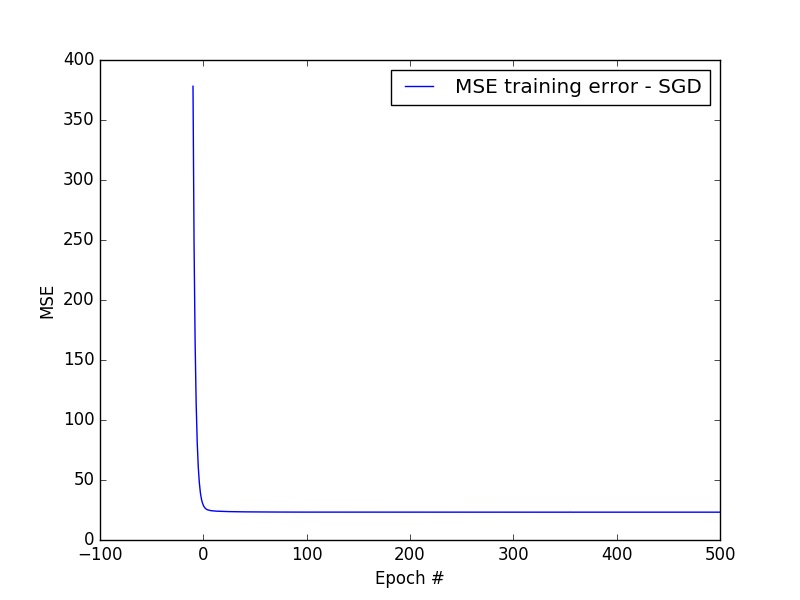
\includegraphics[width=10cm]{MSE_training_error_SGD.jpg}
\caption{Graph showing the MSE training error when using SGD}
\end{figure}

\item For part c) we compute the batch gradient descent to train our model. The learned weight vector is \[\left[\begin{matrix}22.94100877  &-0.93633622   1.18953456 &  0.21723452 &  0.66970526&
  -2.10547565 \\  2.75126807  & 0.30756426  &-3.12381189  & 2.95817231
  -2.4511536 \\  -2.00722057 &  0.90553088 & -4.05729245 \end{matrix}\right]\]
  where this last expression is just one $14 \times 1$ vector.\\
 From this weight vector, we can see that the \textbf{bias term} is $22.94100877$.\\

The \textbf{training errors} (the MSE for training data ) is $23.191557895$, while the \textbf{test errors} (the MSE for test data) is $10.9611791412$.\\

 Finally, we can see the plot of the training error at the end of each epoch in figure 2 below.

\begin{figure}[h]
\centering
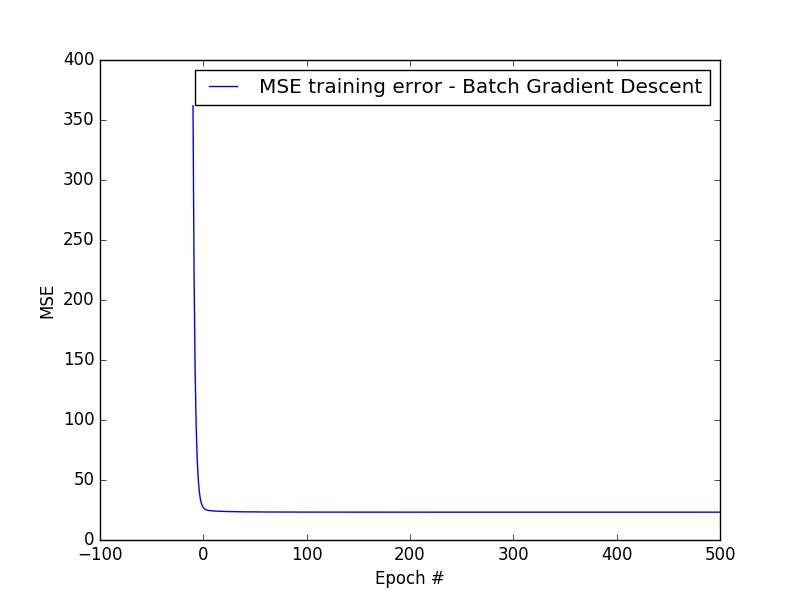
\includegraphics[width=10cm]{MSE_training_error_BGD.jpg}
\caption{Graph showing the MSE training error when using BGD}
\end{figure}

\item In this part of the problem, we use the close solution to identify the weights and bias that minimize the MSE. The weight vector we obtain from using the closed form solution is \[\left[ \begin{matrix} 22.94100877 & -0.93652728   1.18983479 &  0.2180906 &   0.66954197&
  -2.10545149  \\ 2.75102471  & 0.30777503 & -3.12356704  & 2.96148512 &
  -2.45469868 \\ -2.00737039 &  0.90552685 & -4.05749492\end{matrix}\right] \] (which again is a $14 \times 1$ vector but for the sake of space we wrote it as above) and from this expression we can see that the \textbf{bias that minimzes} the MSE is $22.94100877$. Furthermore, from running the code, we see that The \textbf{training errors} (the MSE for training data ) is $23.1915564692$, while the \textbf{test errors} (the MSE for test data) is $10.9665431668$.\\ From tese computations, we can see that the closed form parameters agree very closely with the ones we comptued in the previous part. 

\item After computing the random train and test splits we obtained the following mean training error $21.8527415202$ and the mean test error $23.3165328596$

\end{enumerate}
\end{problem}

\begin{problem}
\normalfont
\begin{enumerate}
\item In the first of the problem, we get the following RMSE errors:
\begin{itemize}
\item $0$th training RMSE: $9.48269466477$
\item $0$th test RMSE: $5.99400813094$
\item $1$-th training RMSE: $4.81576125542$
\item $1$-th test RMSE: $3.3115771419$
\item $2$-th training RMSE: $3.76629417811$
\item $2$-th test RMSE: $7.14746413377$
\item $3$-th training RMSE: $8.18681202323$
\item $3$-th test RMSE: $12.1042413766$
\item $4$-th training RMSE:$8.50491214305$
\item $4$-th test RMSE:$141.55345743$
\end{itemize} 

Finally, we can also see the plot of these values in the followin graph (Figure 3):

\begin{figure}[h]
\centering
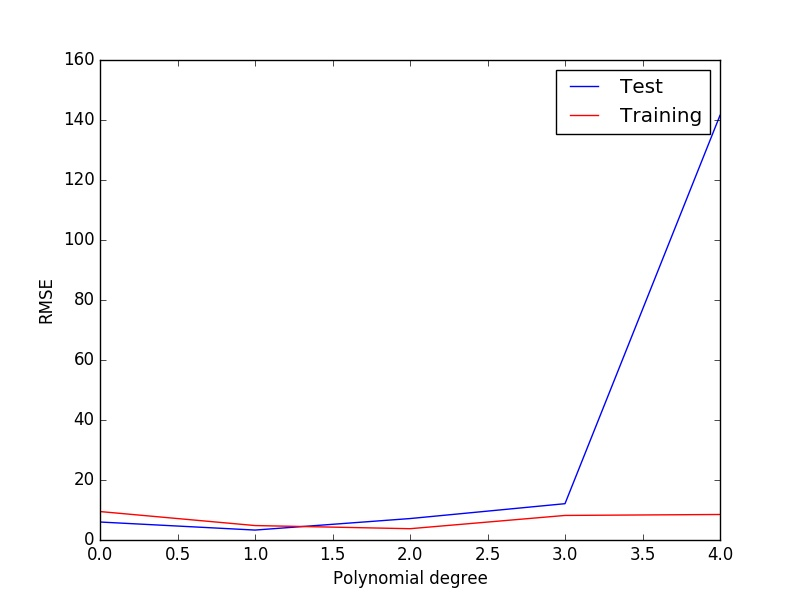
\includegraphics[width=10cm]{HWP2_all_RMSE_degree.jpg}
\caption{Graph showing the MSE error when doing polynomial features of different degrees}
\end{figure}

Since the last part of the graph is not very logical, to appreciate better the graph, we can just graph all elements except the last one, which we can see in Figure 4:

\begin{figure}[!htbp]
\centering
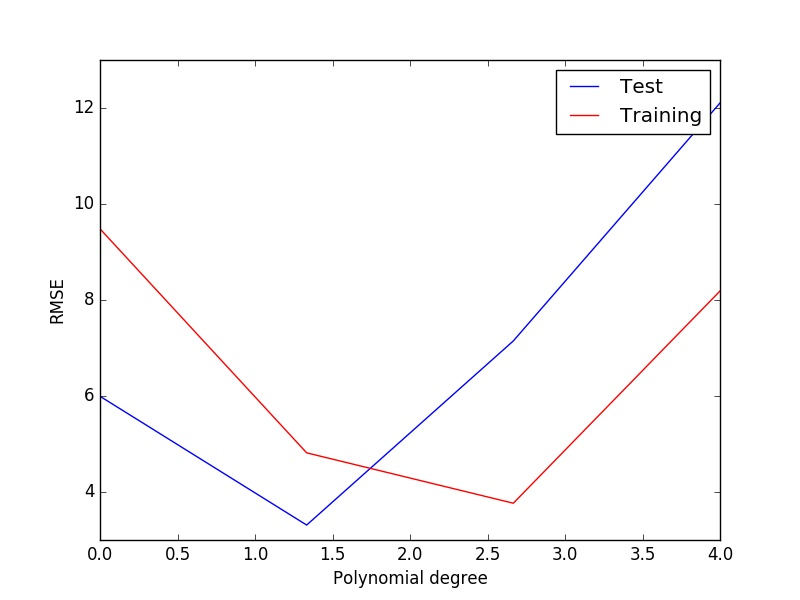
\includegraphics[width=10cm]{HWP2_MSE_except_one.jpg}
\caption{Graph showing the MSE error when doing polynomial features of different degrees, just removing the last value}
\end{figure}

\item Finally, we get the following results for when we restrict the training set and start growing:

\begin{itemize}

\item This is the RMSE for training with 20\% data $11.4601626769$
\item This is the RMSE for test with 20\% data $38.918275945$
\item This is the RMSE for training with 40\% data $2.96802006698$
\item This is the RMSE for test with 40\% data  $9.32135308145$
\item This is the RMSE for training with 60\% data $3.14261785825$
\item This is the RMSE for test with 60\% data $7.57749760854$
\item This is the RMSE for training with 80\% data $3.25304667758$
\item This is the RMSE for test with 80\% data $4.52585085547$
\item This is the RMSE for training with 100\% data $4.81576125542$
\item This is the RMSE for test with 100\% data $3.3115771419$

\end{itemize}

Again, we can visualize this information as shown in Figure 5:

\begin{figure}[!htbp]
\centering
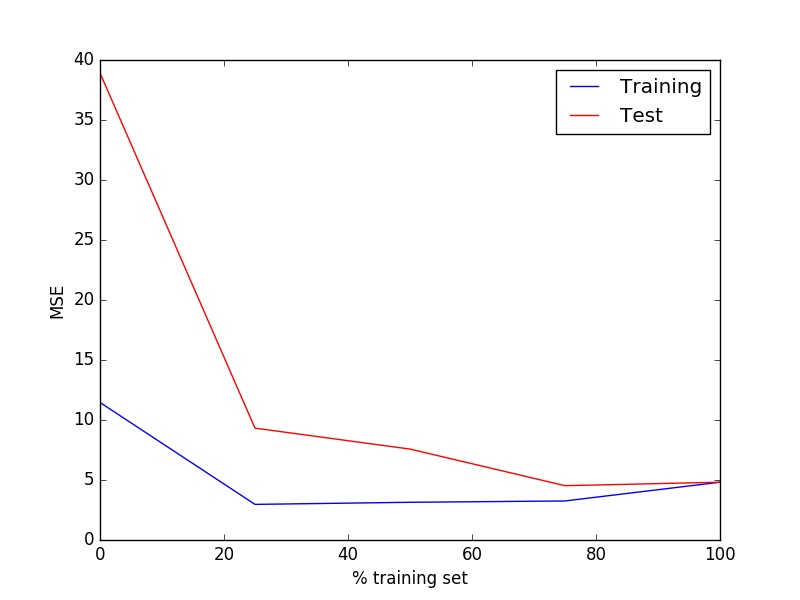
\includegraphics[width=10cm]{HWp2_Percentag_train.jpg}
\caption{Graph showing the MSE error for training and test data when changing the available percentage of data.}
\end{figure}
\end{enumerate}
\end{problem}

\begin{problem}
\normalfont
\begin{enumerate}
\item For this first problem, we show the work done in FIgure 6:

\begin{figure}[!htbp]
\centering
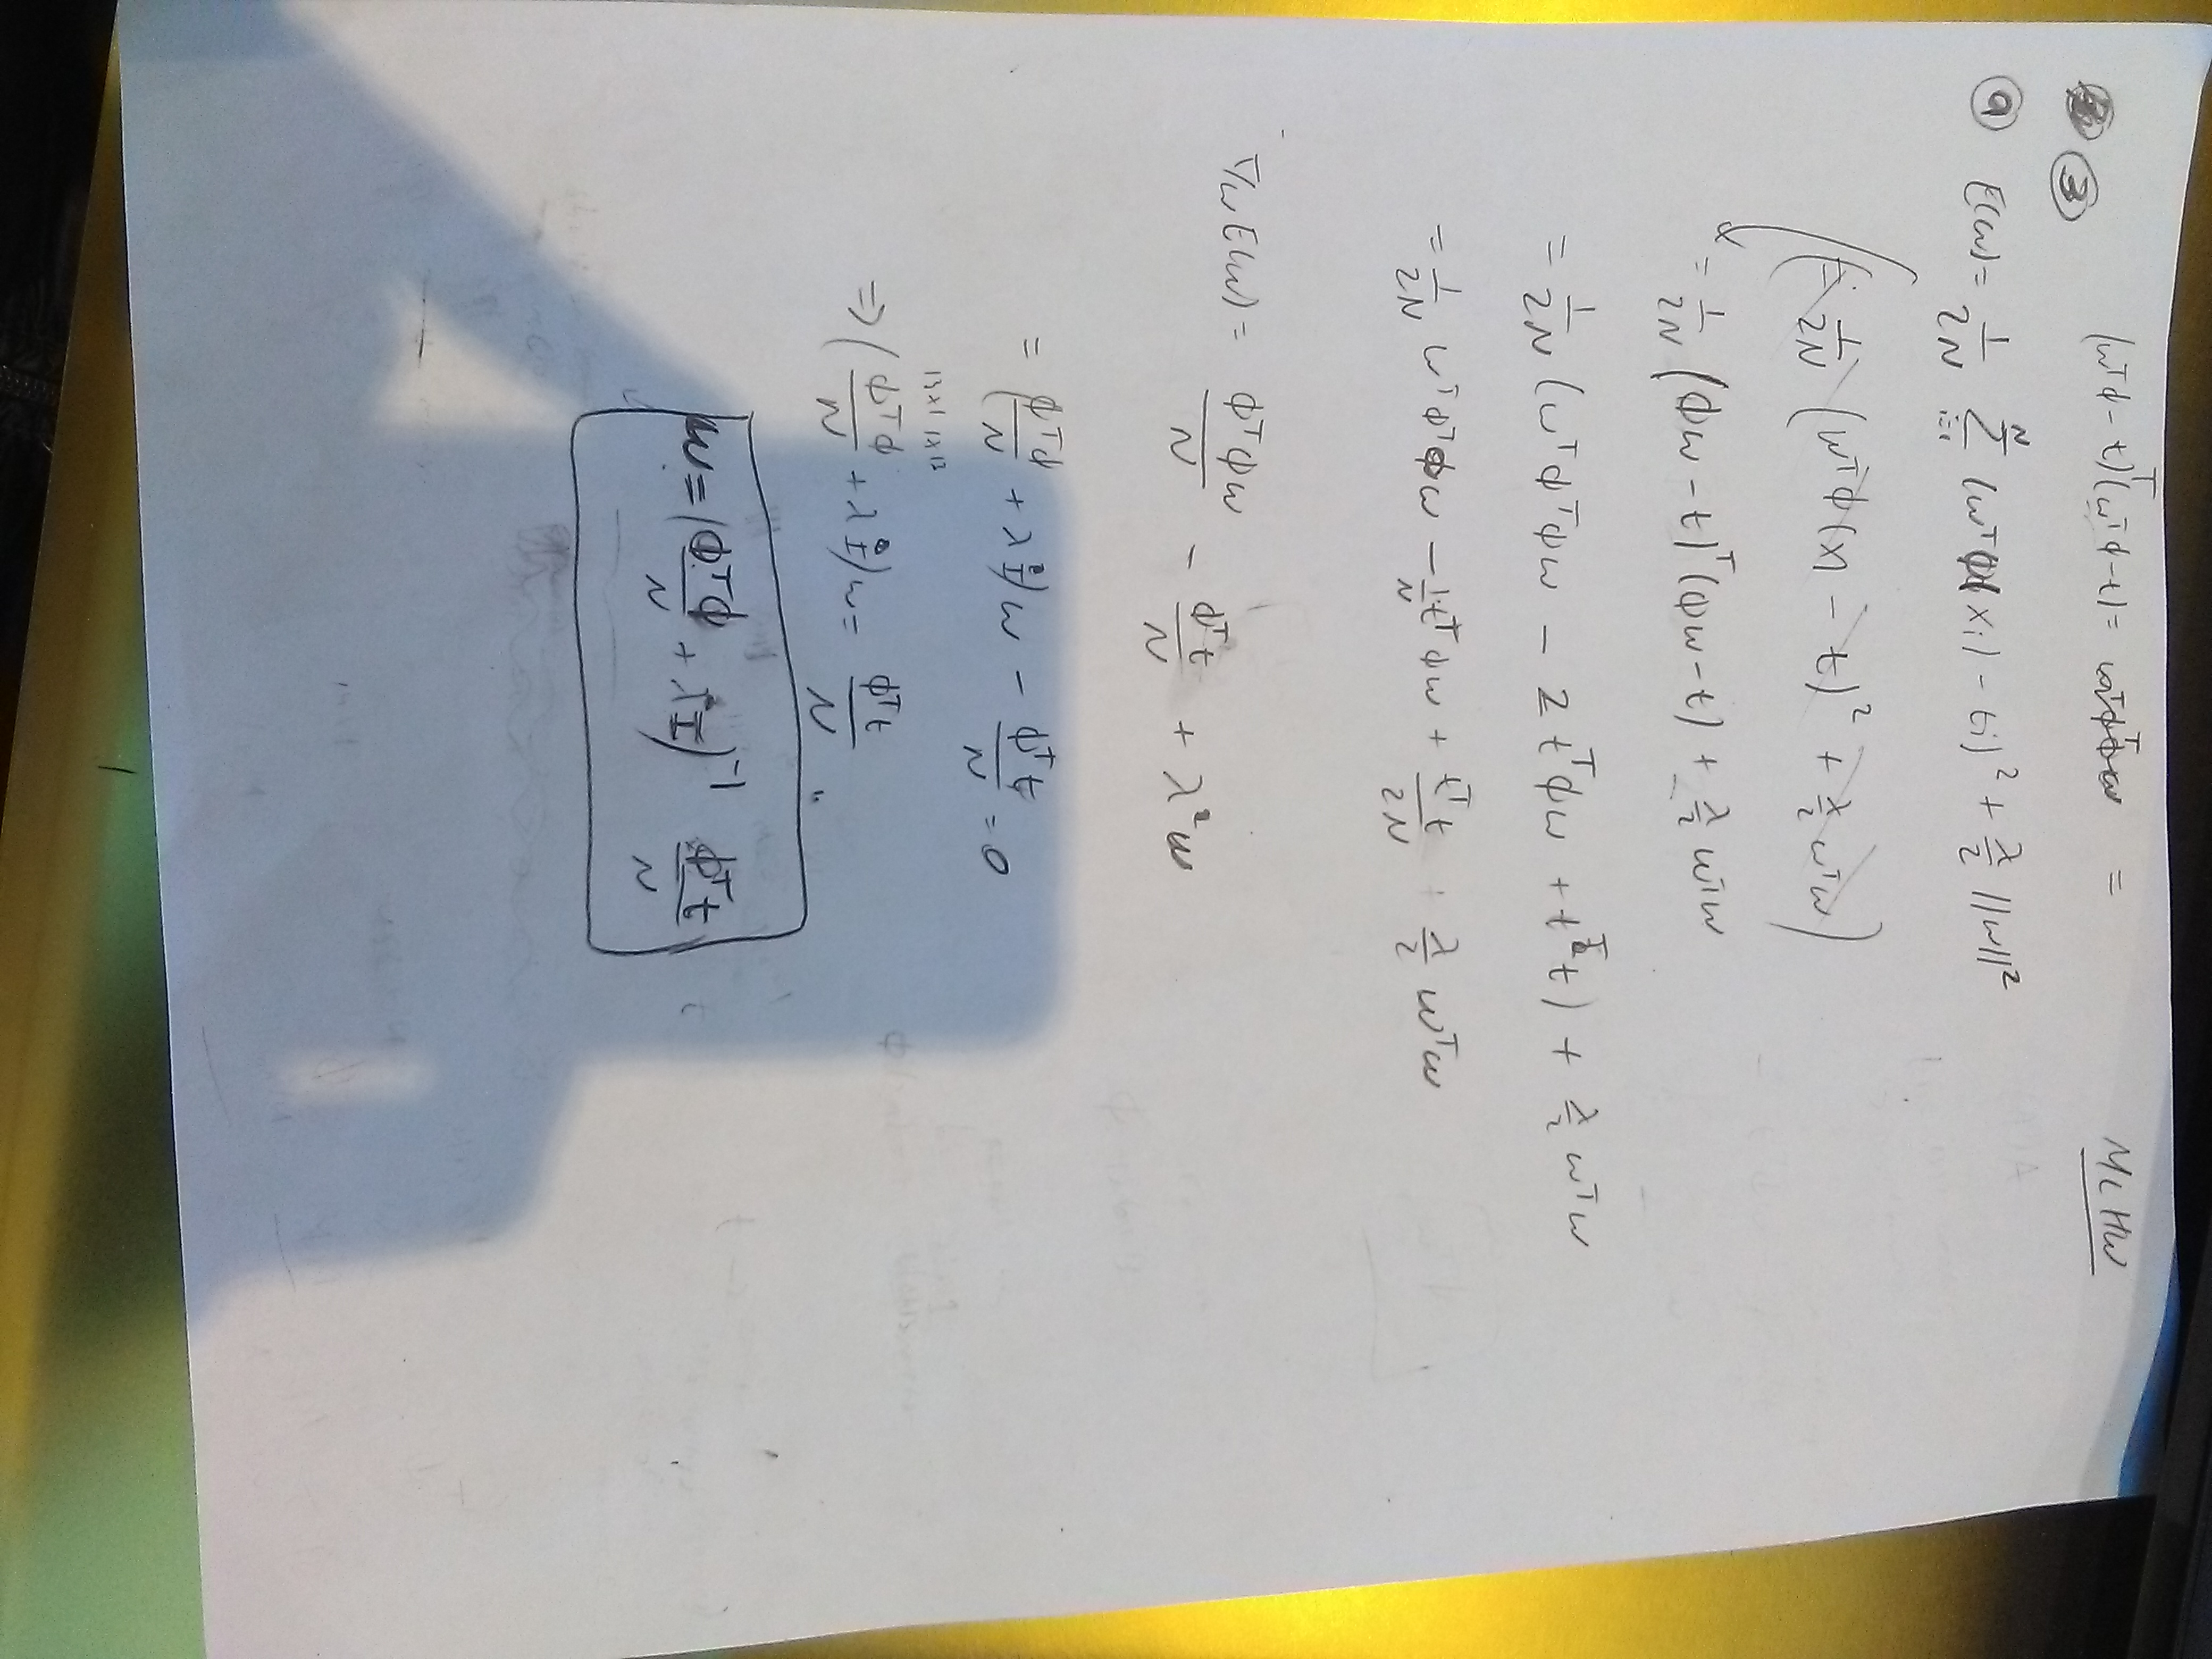
\includegraphics[width=15cm, angle = 90]{Problem3a.jpg}
\caption{Image showing how we computed the closed form solution of the regularization problem in problem 3a.}
\end{figure}

\item FOr this problem we repport all the possible RMSE, namely validation, training and test set for the possible lambdas:

\begin{itemize}
\item The RMSE error of training set with $\lambda = 0$ is $4.75899856011$
\item The RMSE error of validation set with $\lambda = 0$ is $7.84564027897$
\item The RMSE error of test set with $\lambda = 0$ is $4.22655365439$
\item The RMSE error of training set with $\lambda = 0.1$ is $5.31569487929$
\item The RMSE error of validation set with $\lambda = 0.1$ is $5.49507024934$
\item The RMSE error of test set with $\lambda = 0.1$ is $3.18380156819$
\item The RMSE error of training set with $\lambda = 0.2$ is $6.37532816836$
\item The RMSE error of validation set with $\lambda = 0.2$ is $4.54395472308$
\item The RMSE error of test set with $\lambda = 0.2$ is $3.92160042074$
\item The RMSE error of training set with $\lambda = 0.3$ is $7.51722511924$
\item The RMSE error of validation set with $\lambda = 0.3$ is $4.48444830133$
\item The RMSE error of test set with $\lambda = 0.3$ is $5.11613124943$
\item The RMSE error of training set with $\lambda = 0.4$ is $8.60568912038$
\item The RMSE error of validation set with $\lambda = 0.4$ is $4.93033974684$
\item The RMSE error of test set with $\lambda = 0.4$ is $6.29716462016$
\item The RMSE error of training set with $\lambda = 0.5$ is $9.60402790097$
\item The RMSE error of validation set with $\lambda = 0.5$ is $5.57508121459$
\item The RMSE error of test set with $\lambda = 0.5$ is $7.36843458243$
\end{itemize}

Furthermore, we see that the lowest RMSE error on the validation set is $ 4.48444830133$ happening on $\lambda = 0.3$. The corresponding test error for this $\lambda = 0.3$ is $5.11613124943$.

Finally, we can see a picture of how the test, validation and training MSE behave for different $\lambda$ in the table below, this picture corresponds to figure 7.

\begin{figure}[!htbp]
\centering
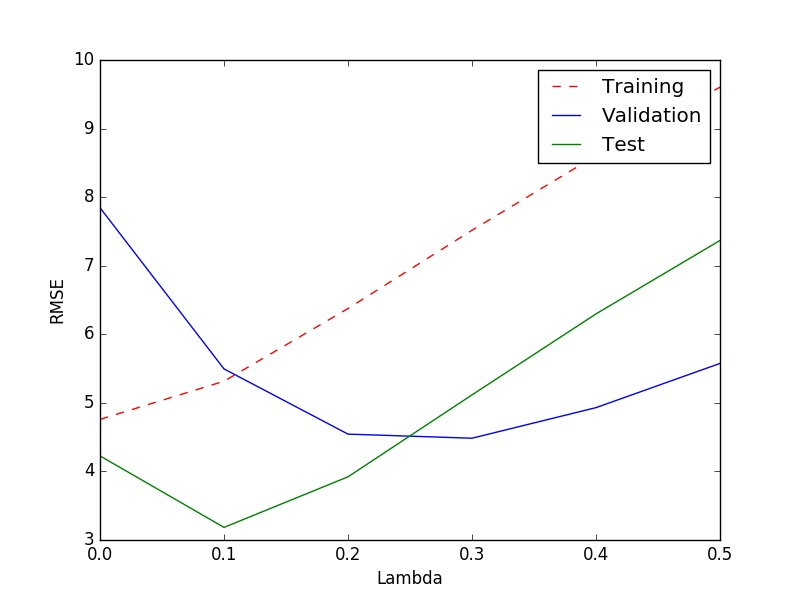
\includegraphics[width=10cm]{Problem3b_lambda.jpg}
\caption{Image showing the behavior of RMSE when we have different regularization parameters.}
\end{figure}

\end{enumerate}
\end{problem}

\begin{problem}
\normalfont
Finally, we show the theoretical in the following scanned pictures, corresponding to Figure 8, 9, 10 and 11.

\begin{figure}[!htbp]
\centering
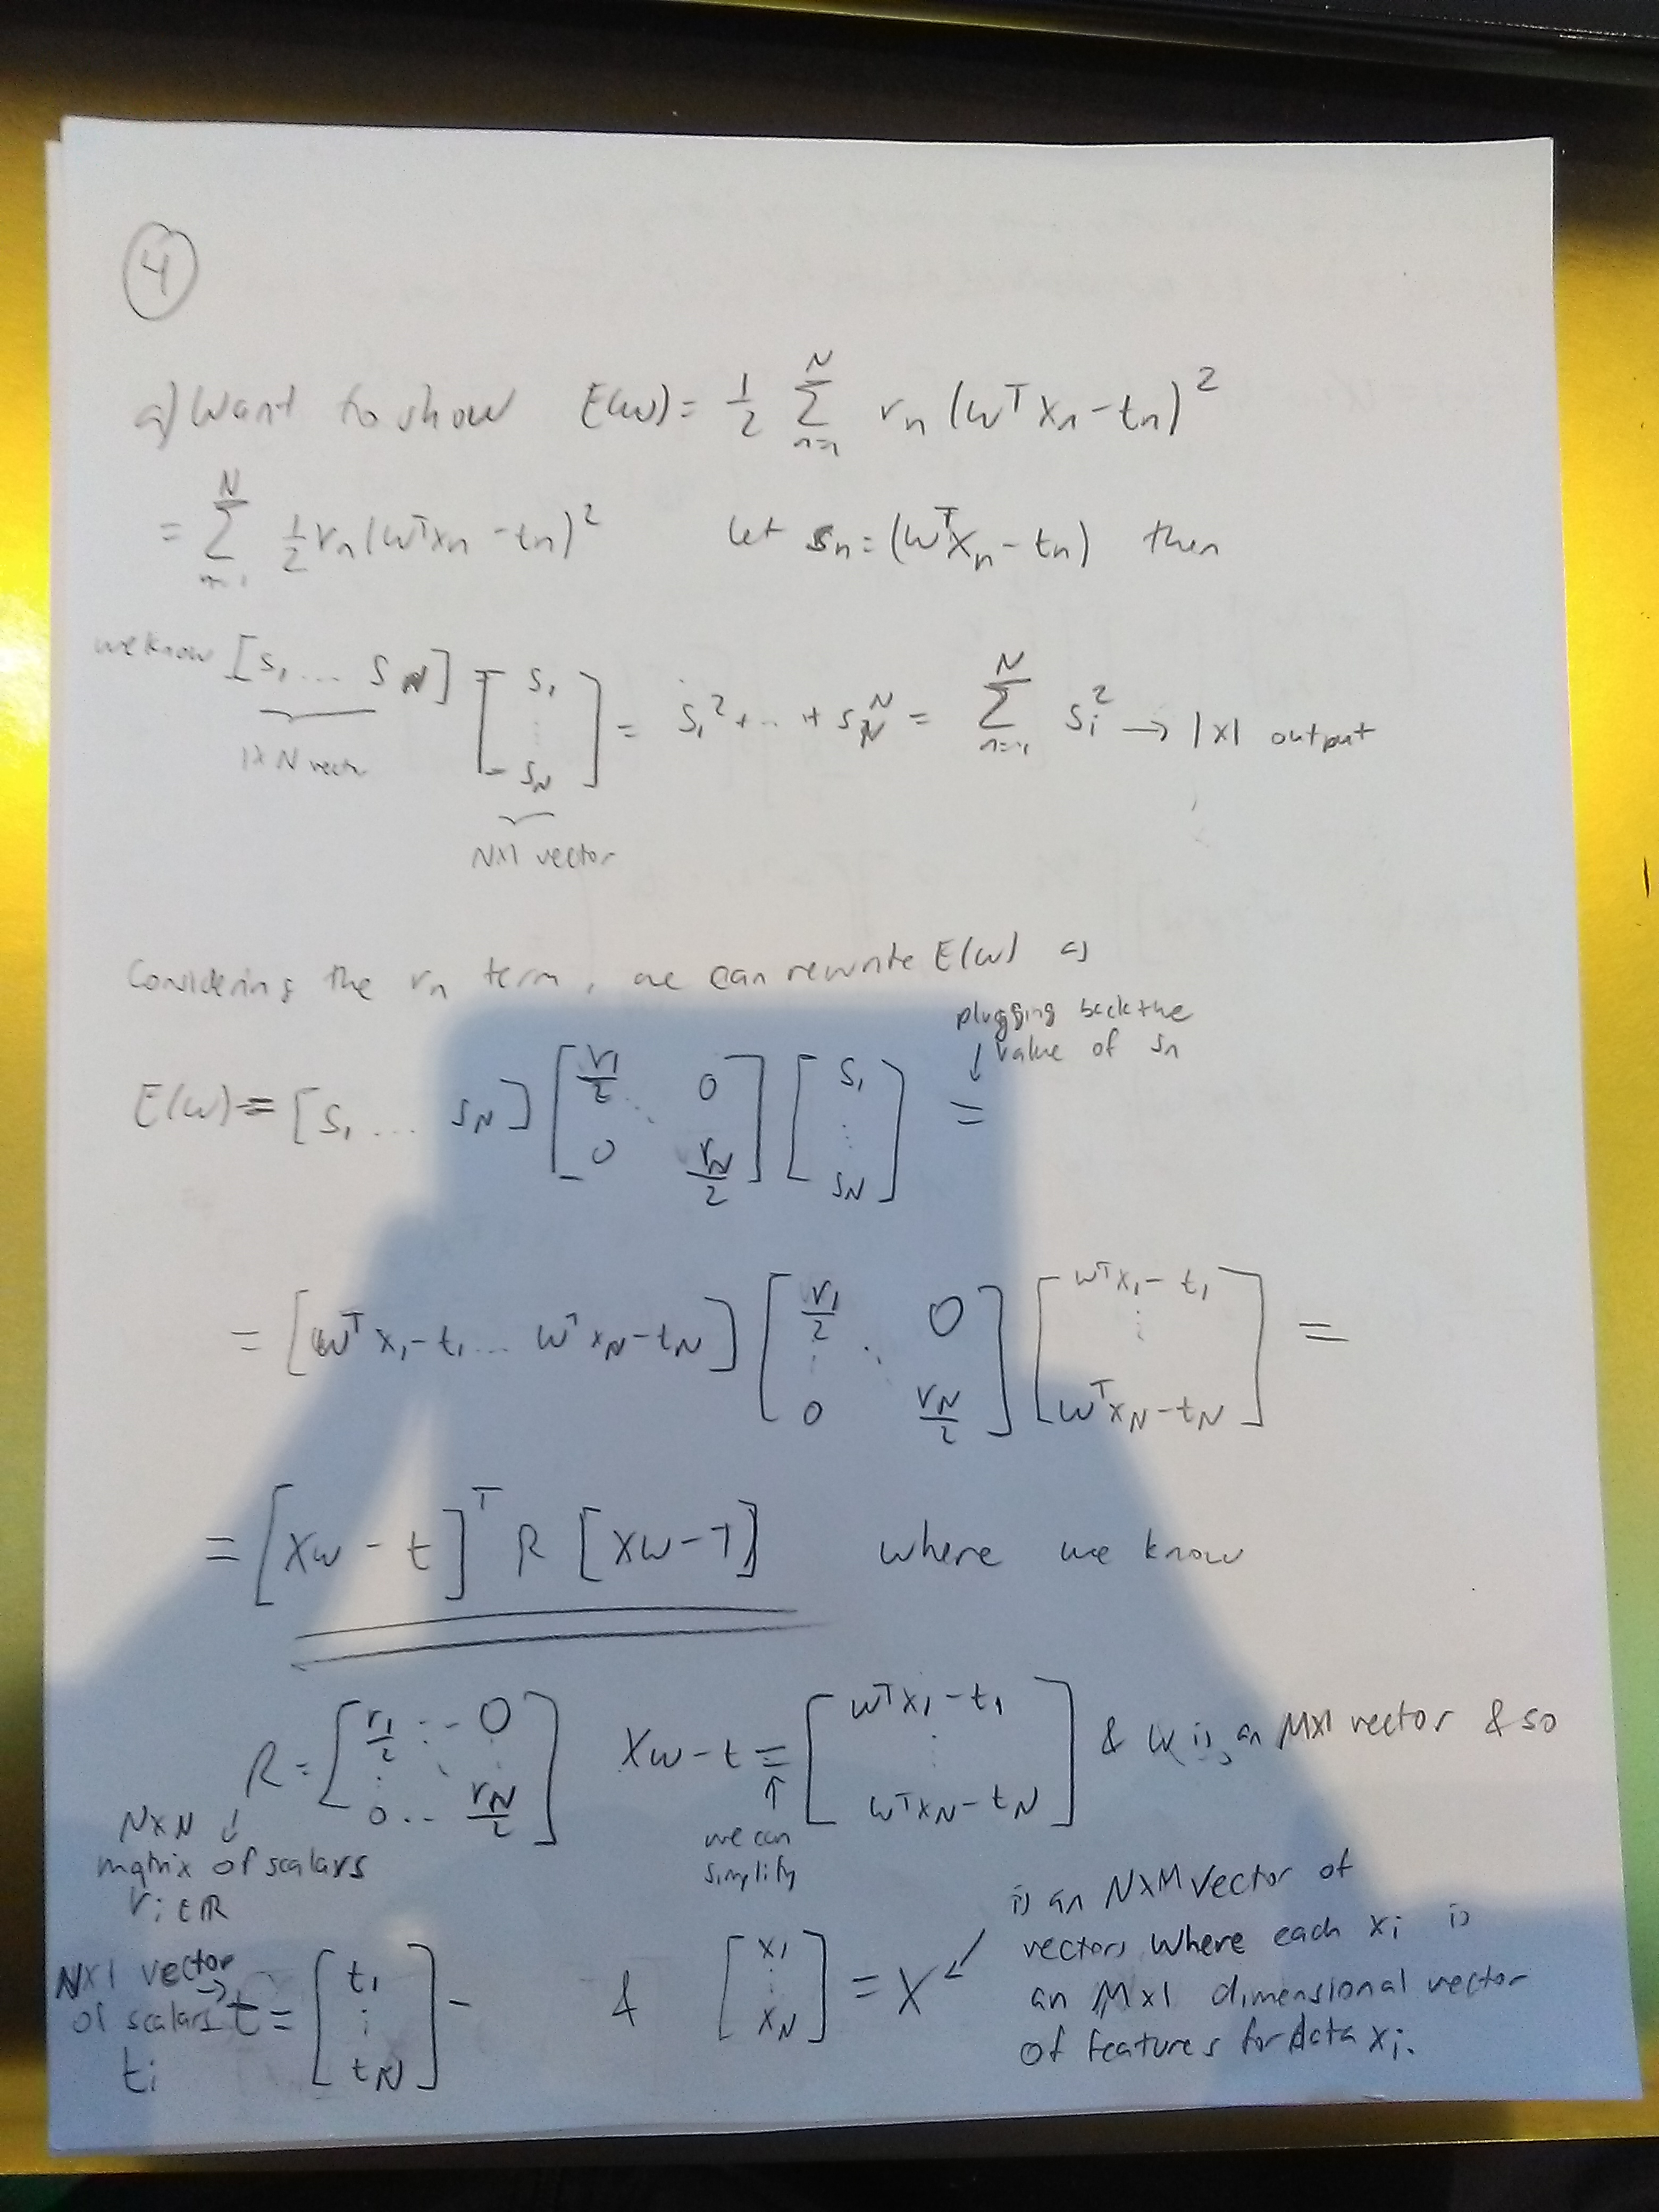
\includegraphics[width=15cm]{Problem4a.jpg}
\caption{Image showing part a of problem 4.}
\end{figure}
\end{problem}

\begin{figure}[!htbp]
\centering
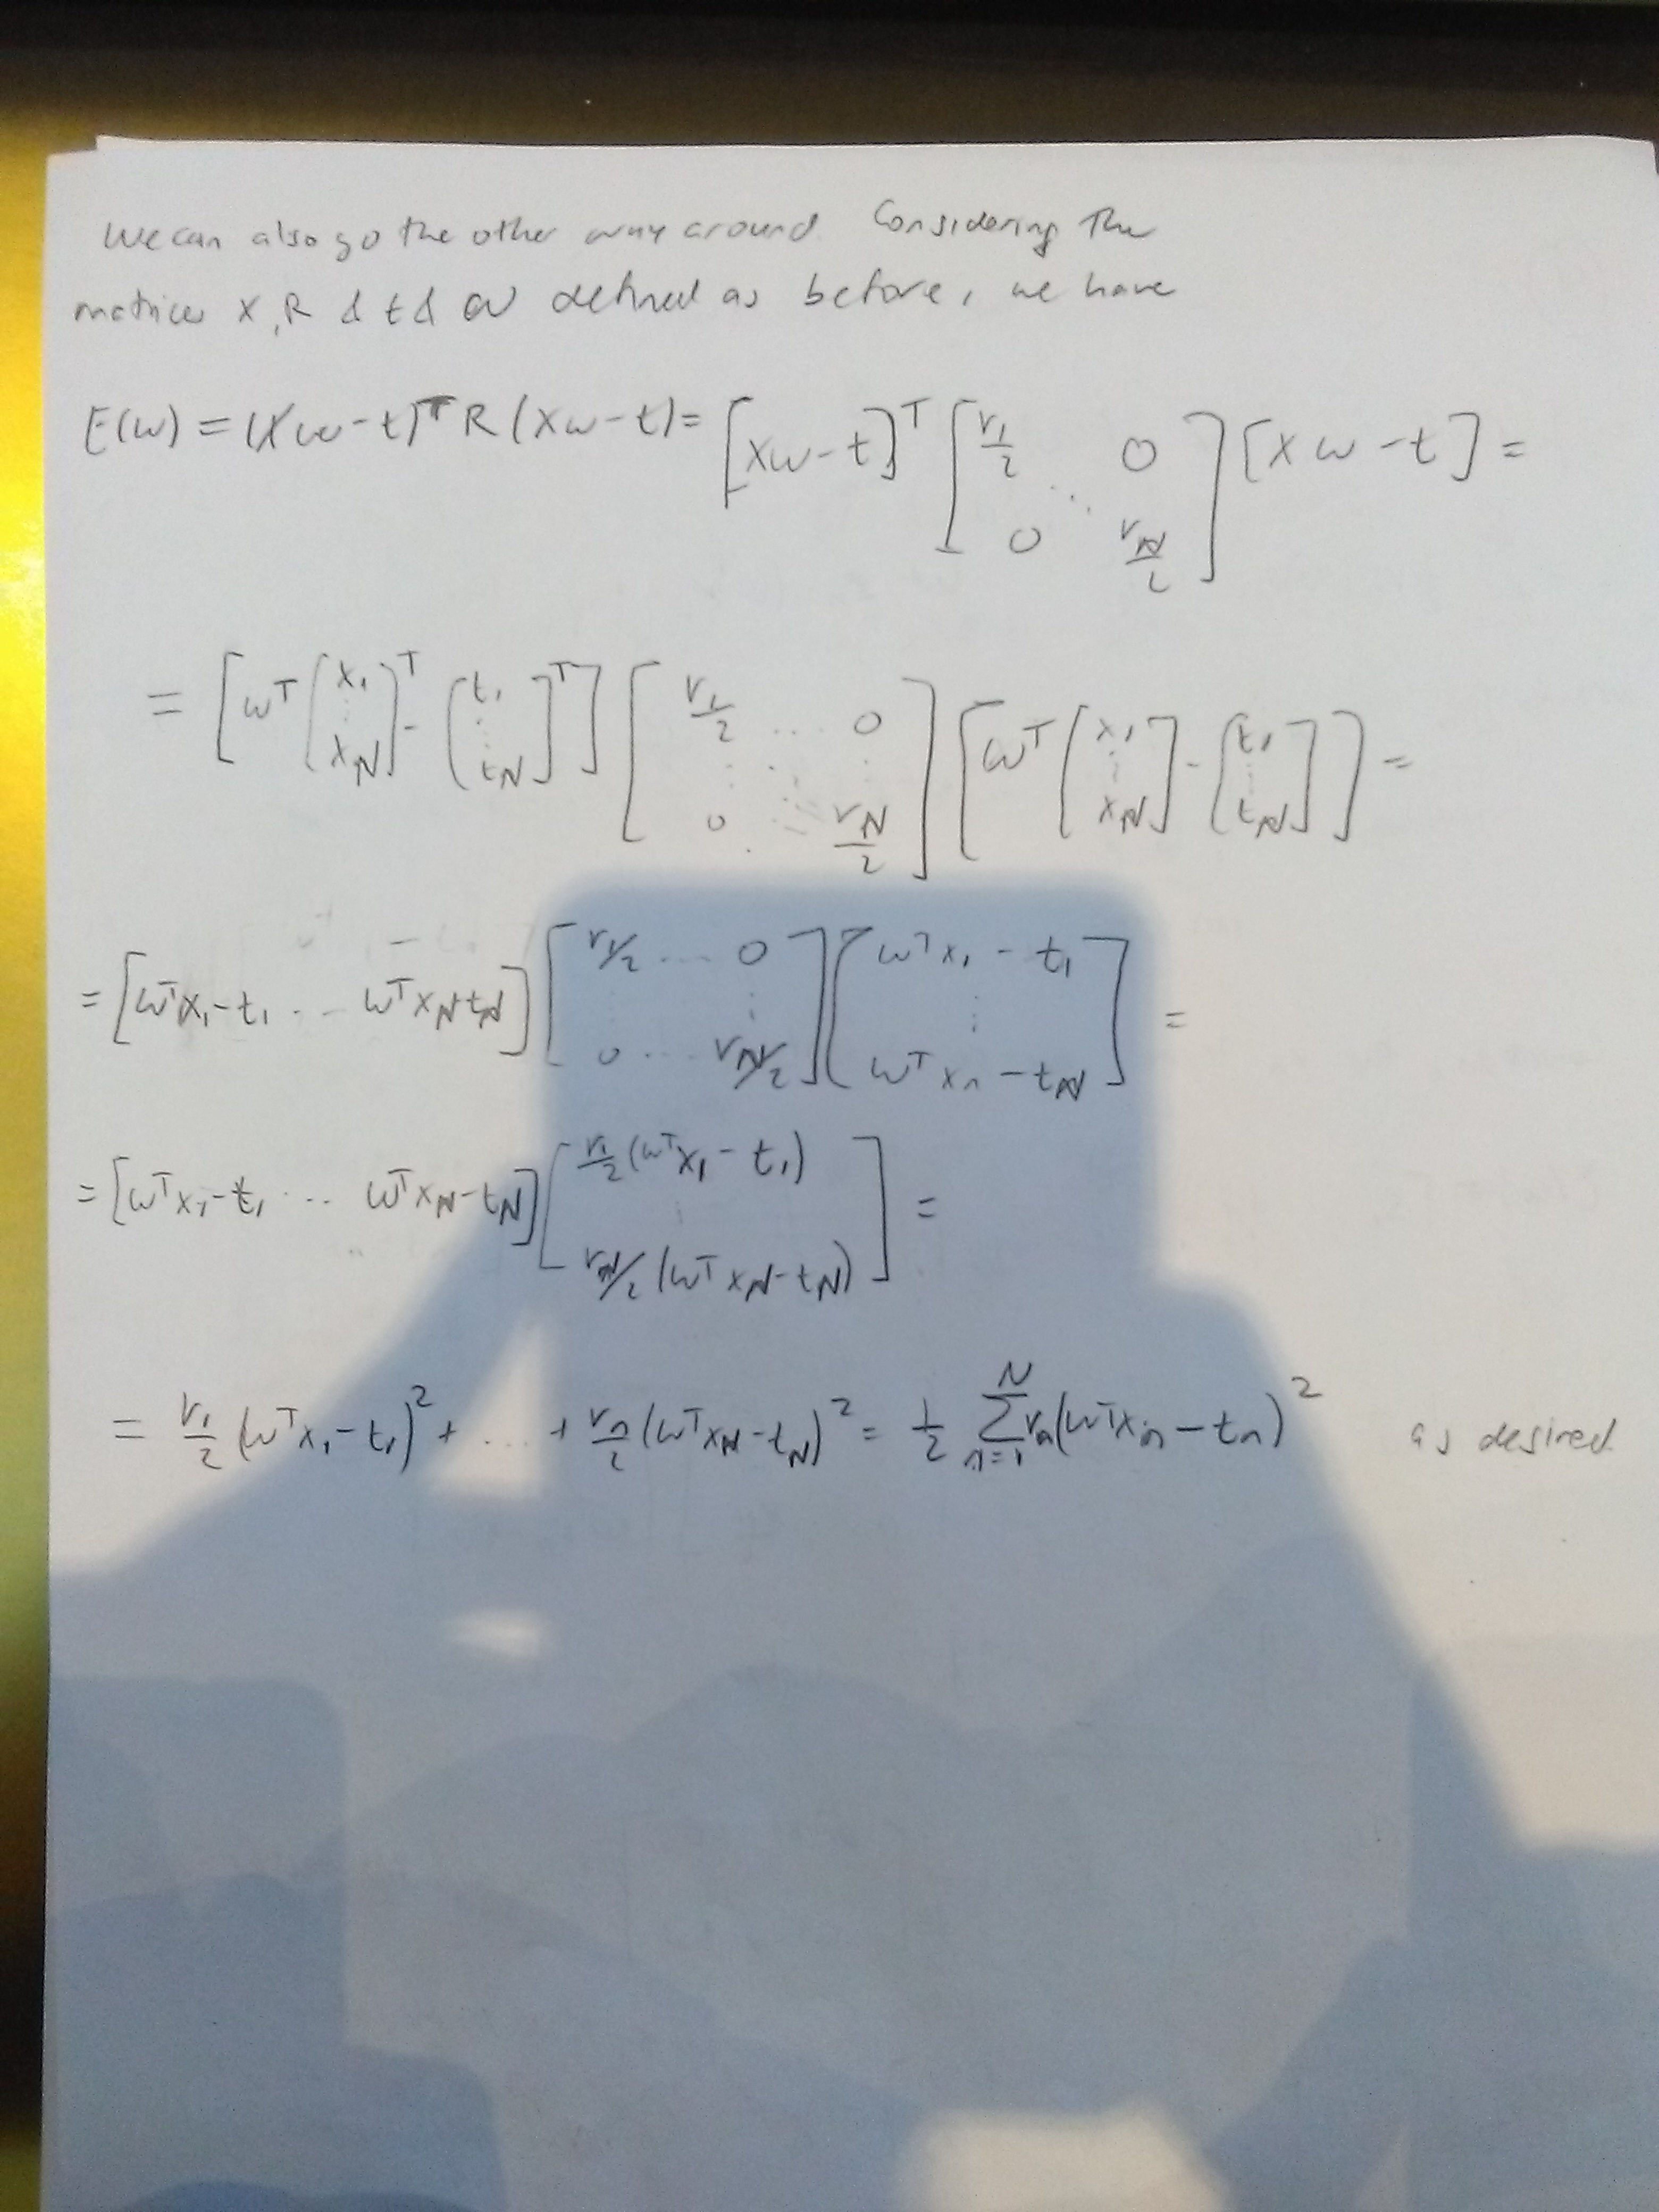
\includegraphics[width=15cm]{problem4a_2.jpg}
\caption{Image showing a continuitation to part a of problem 4a.}
\end{figure}

\begin{figure}[!htbp]
\centering
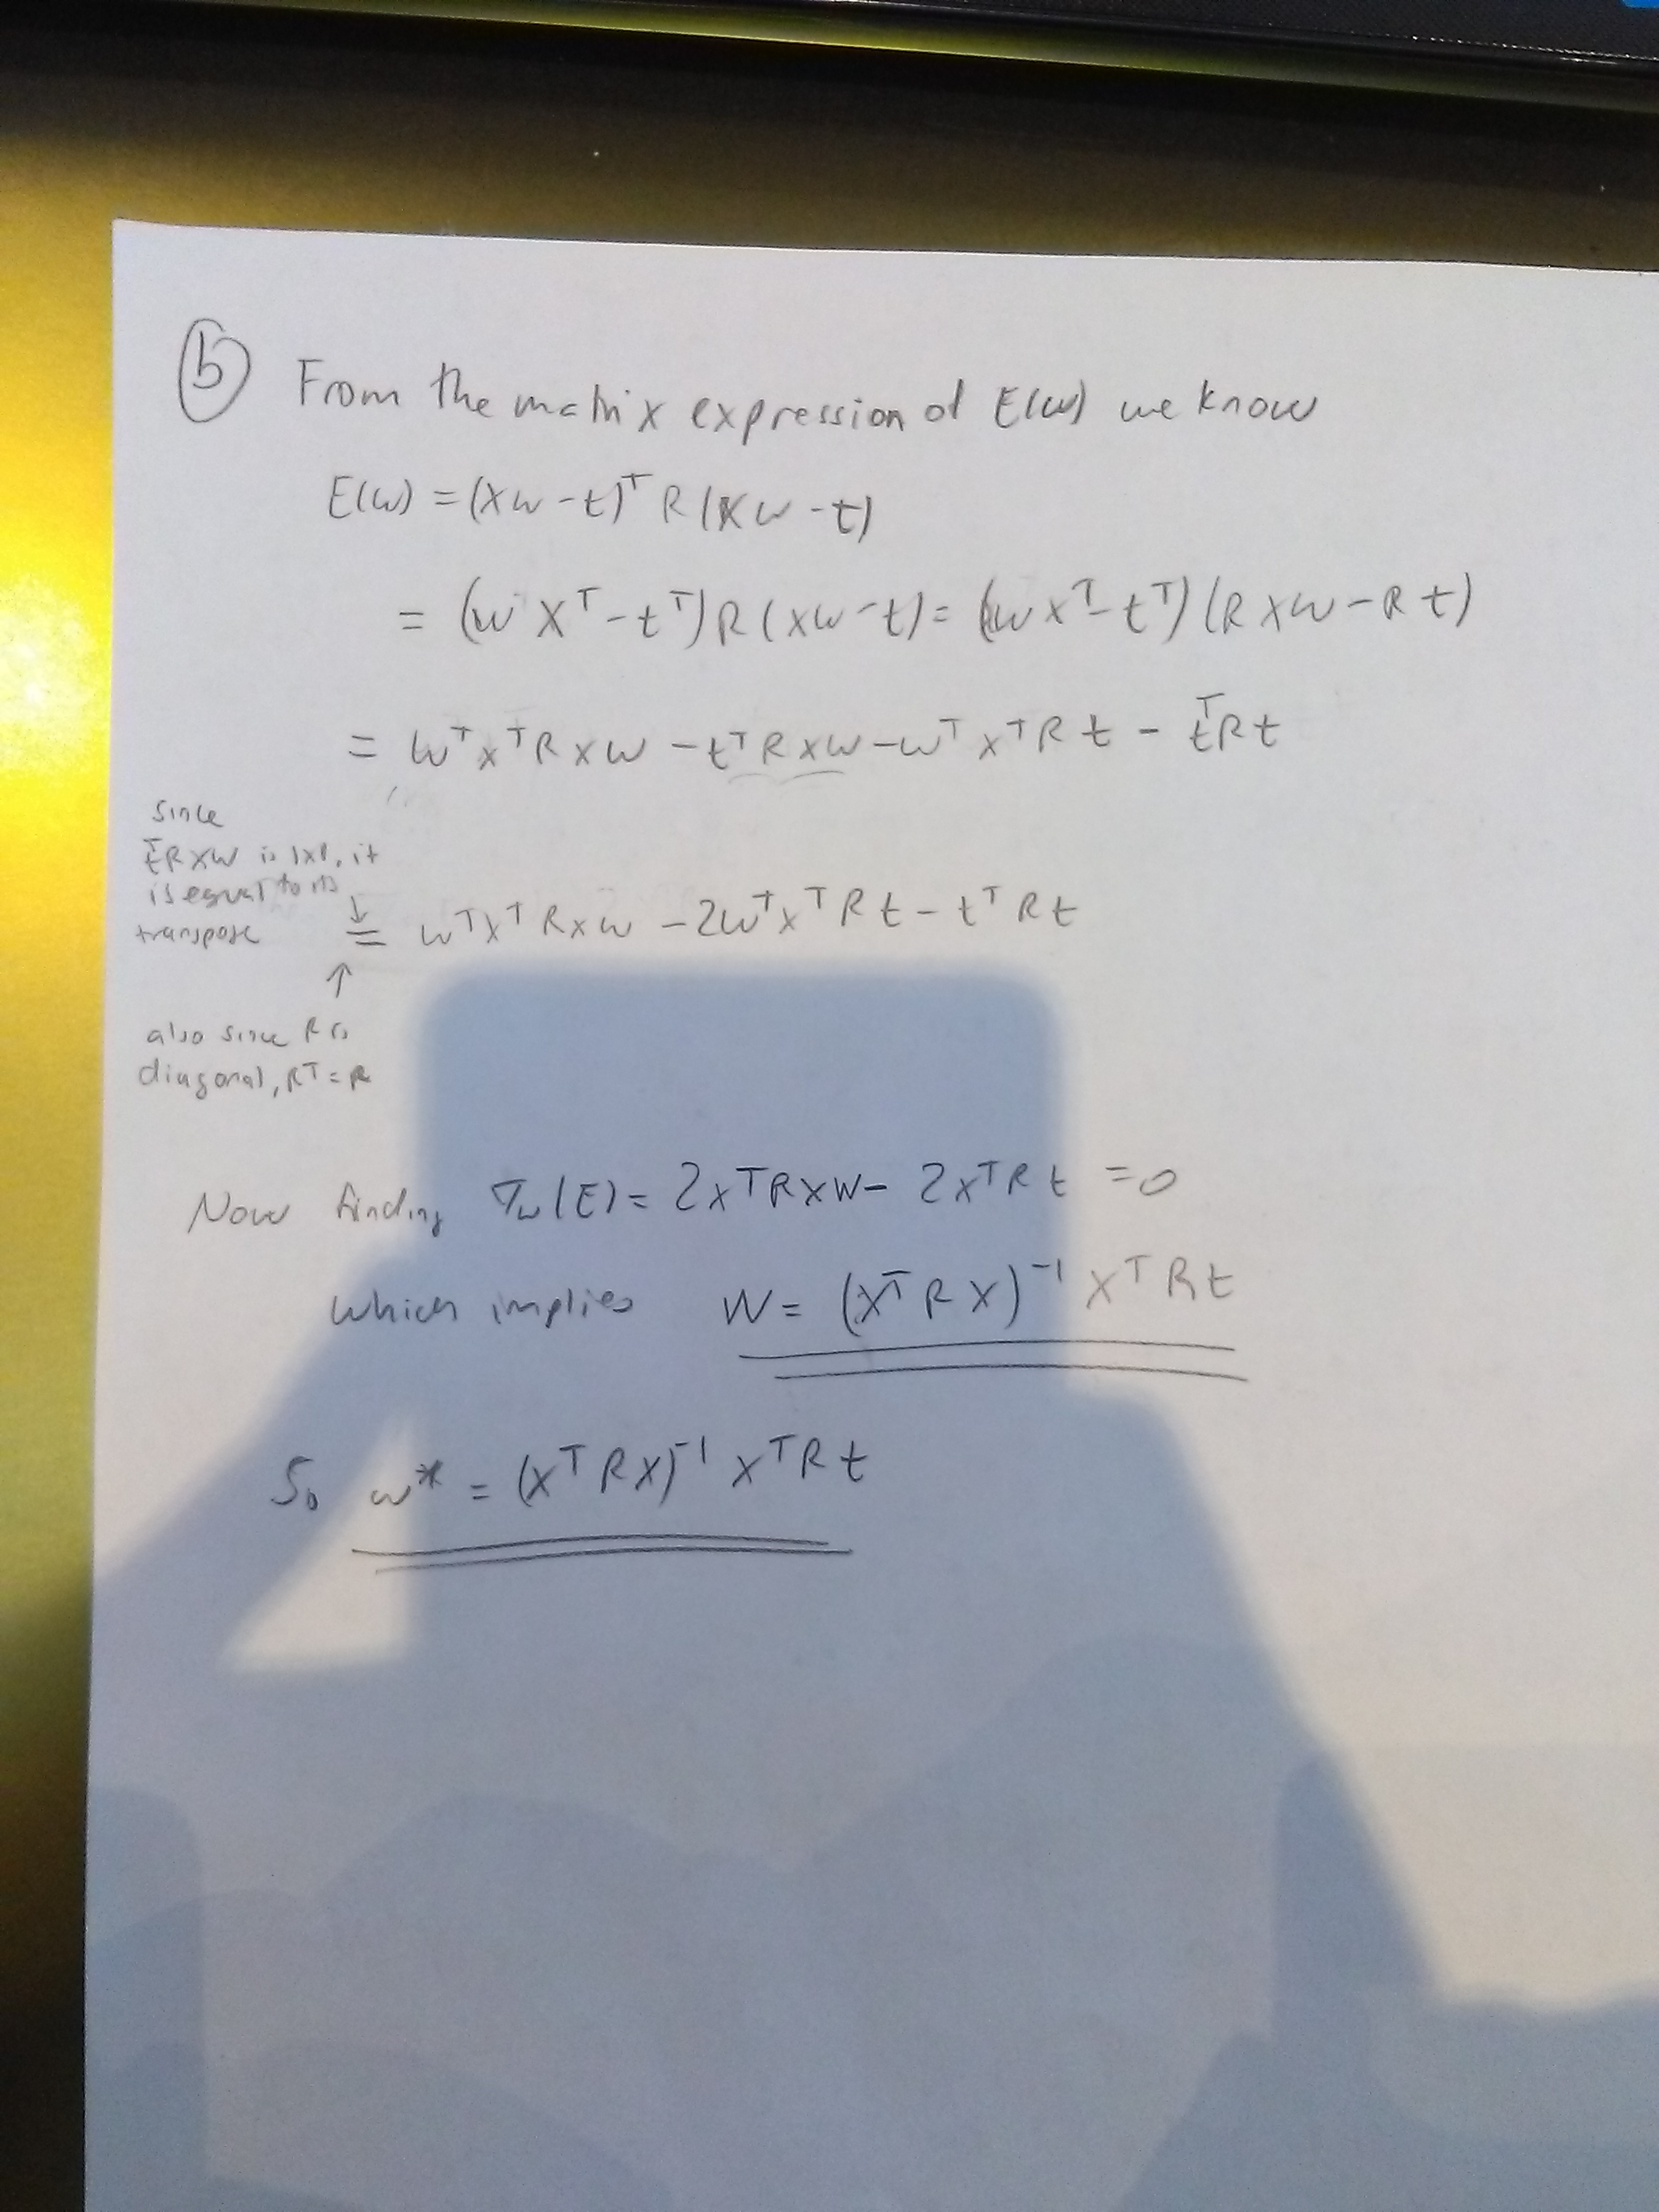
\includegraphics[width=15cm]{problem4b.jpg}
\caption{Image showing the work done to solve problem 4b.}
\end{figure}

\begin{figure}[!htbp]
\centering
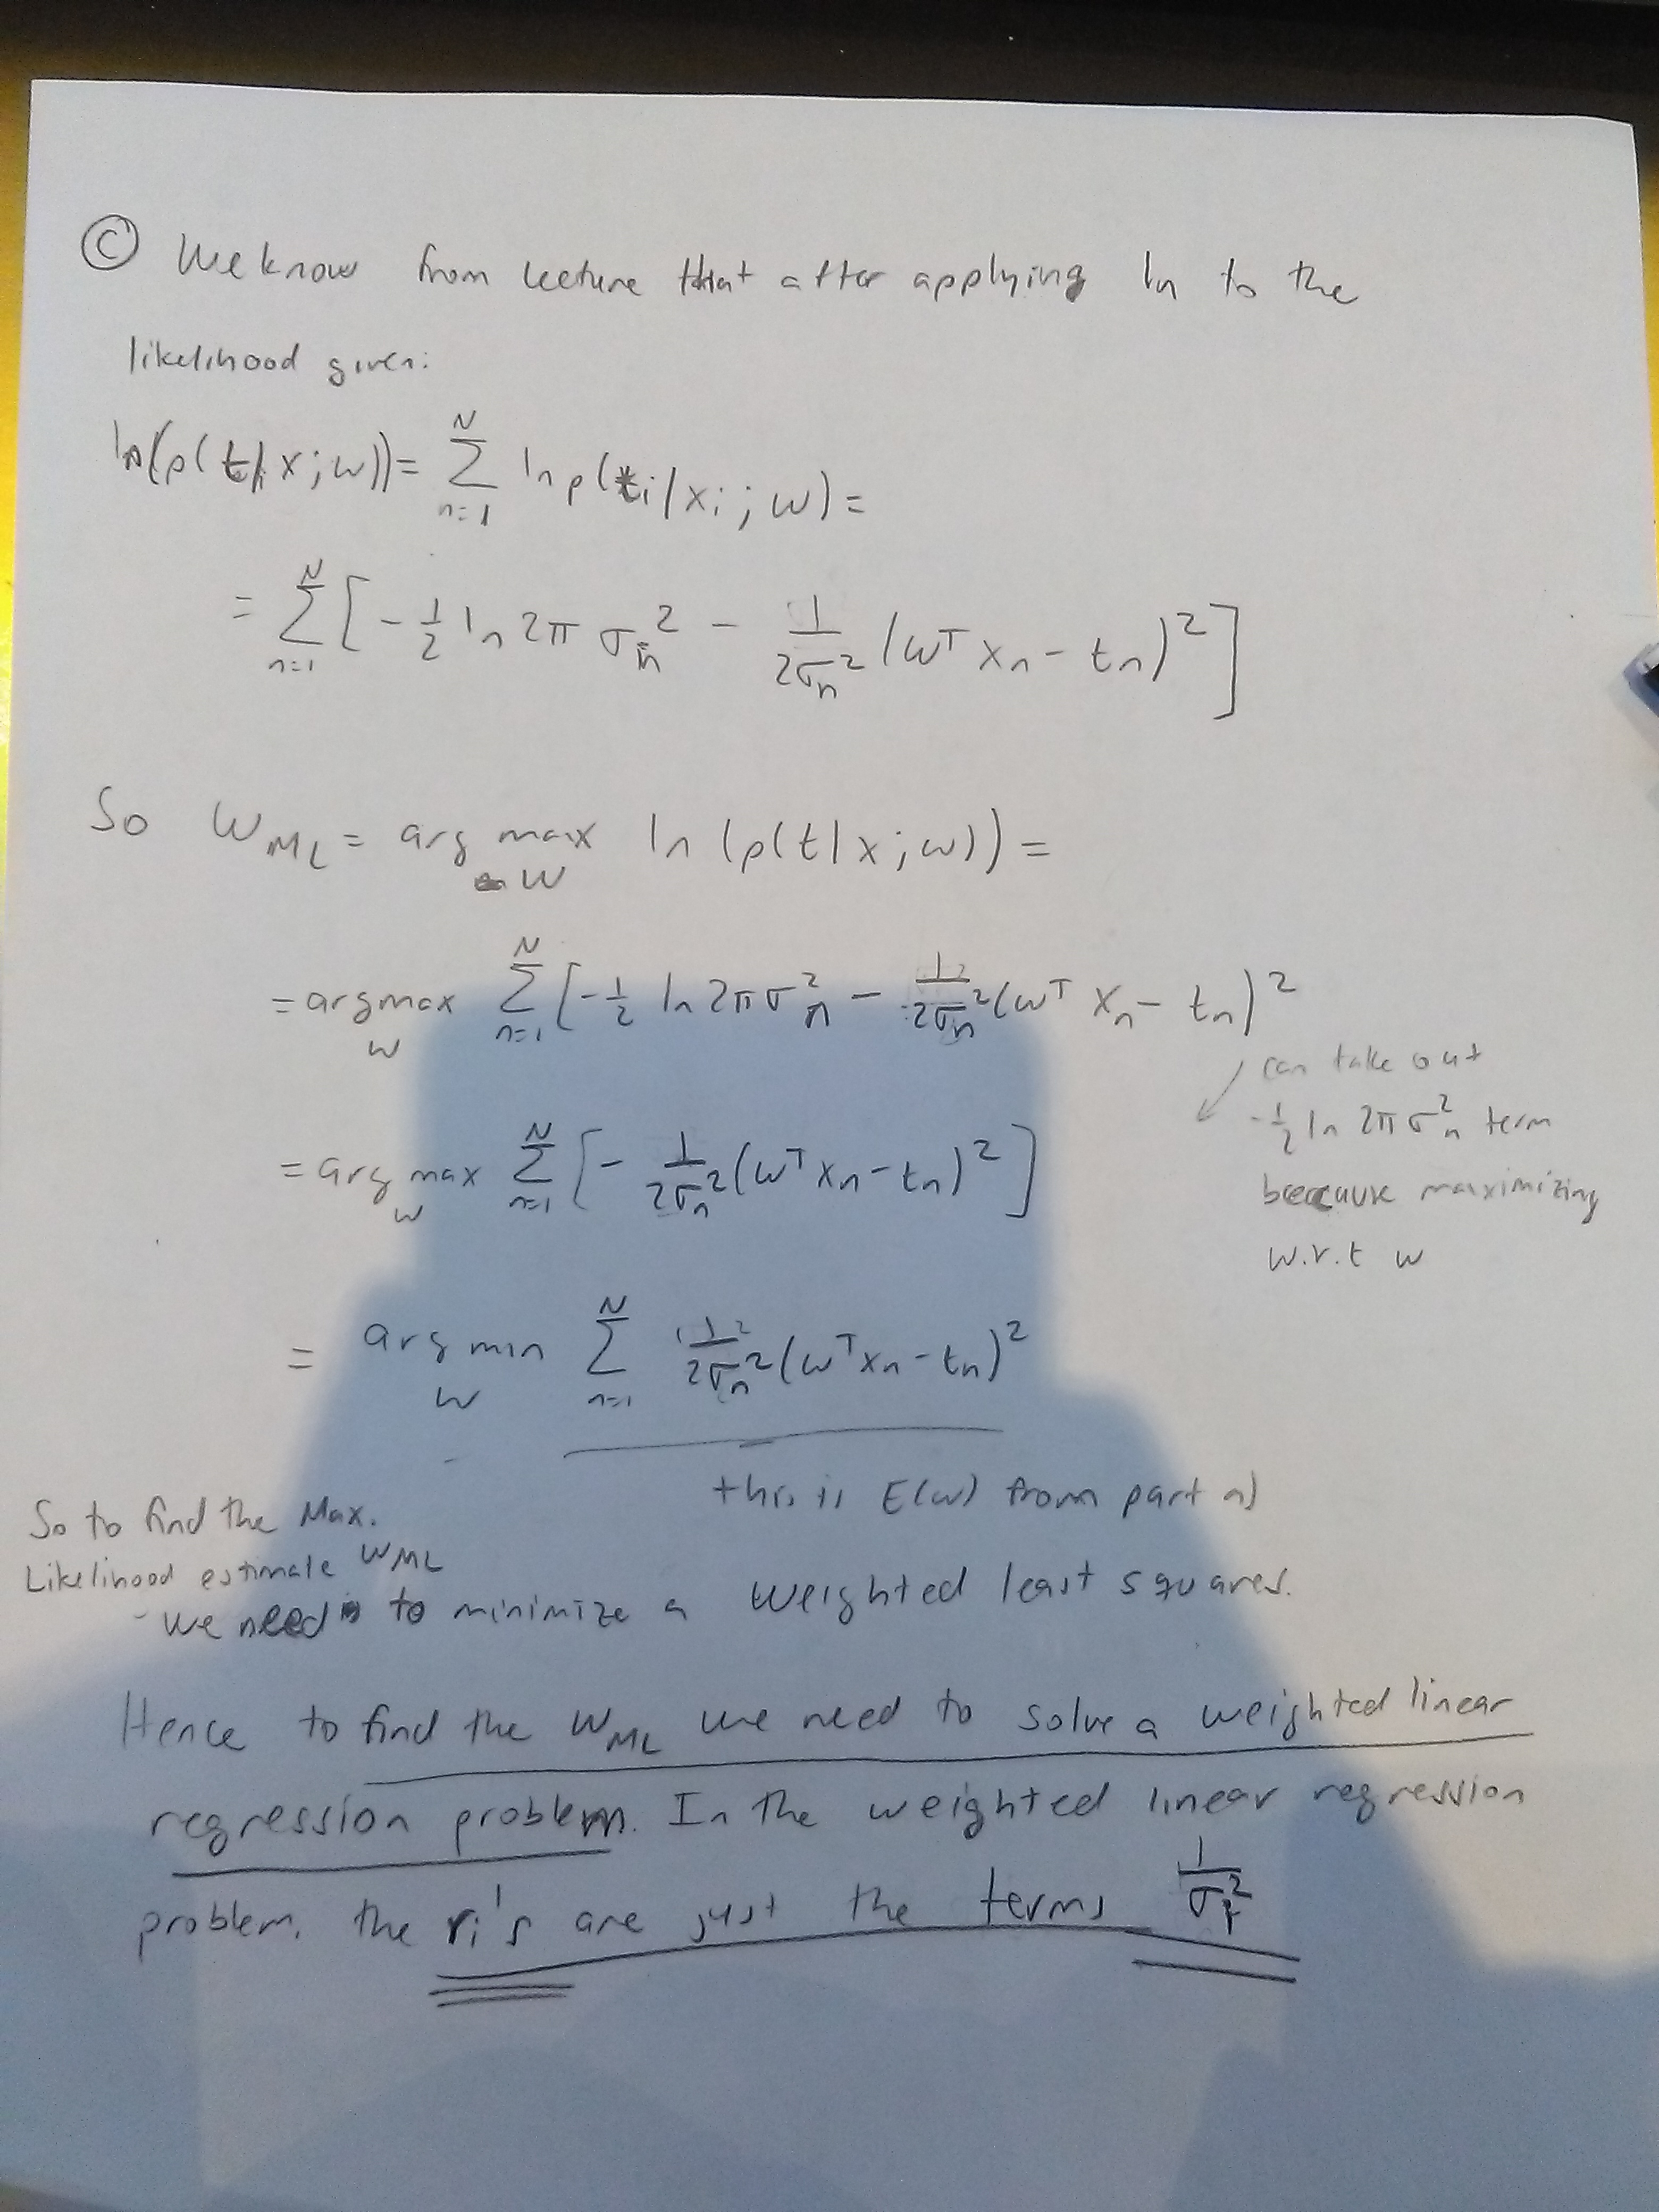
\includegraphics[width=15cm]{Problem_4c.jpg}
\caption{Image showing the work done to find the solution to problem 4c.}
\end{figure}

\end{document}